% network
\documentclass[a4paper, 10pt]{article}
\usepackage[utf8]{inputenc}
\usepackage{t1enc}
\usepackage{times}
\usepackage{fancyhdr}
\usepackage[magyar]{babel}
\usepackage{geometry}
\usepackage{graphicx}
\usepackage{wrapfig}
\usepackage{mathtools}
\usepackage{amssymb}
\usepackage{multicol}
\usepackage{tabularx}
\usepackage{vwcol}
\usepackage{caption}
\usepackage{subcaption}
\usepackage{outlines}
\usepackage{siunitx}
\usepackage{lipsum}
\usepackage{ulem}
\usepackage{rotating}
\usepackage{tikz}
\usepackage{enumitem}
\usepackage{cprotect}
\usepackage{floatrow}
\usepackage[unicode]{hyperref}
\usepackage{import}
\usepackage{xifthen}
\usepackage{pdfpages}
\usepackage{transparent}
\usepackage{xcolor}
\usepackage{listings}
\usepackage{booktabs}
\usepackage{setspace}

\graphicspath{{./figures/}}
\linespread{1.5}
\geometry{margin=3cm}
\floatsetup[table]{capposition=top}

\setlength\parindent{0mm}

\lstset{showstringspaces=false}
\lstset{
	lineskip=1mm,
	language=Python,
	numbers=left,
	tabsize=2,
	numbersep=5mm,
	framexleftmargin=10mm,
	frame=single,
	framerule=0.3mm,
	basicstyle=\footnotesize\ttfamily,
	keywordstyle=\color{blue}\ttfamily\bfseries,
	stringstyle=\color{red}\ttfamily,
	commentstyle=\color{magenta}\ttfamily,
	morecomment=[l][\color{magenta}]{\#}
}

\PassOptionsToPackage{usenames, dvipsnames}{xcolor}
\hypersetup{
  colorlinks   = true, %Colours links instead of ugly boxes
  urlcolor     = blue, %Colour for external hyperlinks
  linkcolor    = blue, %Colour of internal links
  citecolor   = red %Colour of citations
}

\makeatletter
\def\incfig{\@ifnextchar[{\@with}{\@without}}
\def\@with[#1]#2{\def\svgwidth{#1} \import{./figures/}{#2.pdf_tex}}
\def\@without#1{\def\svgwidth{\columnwidth} \import{./figures/}{#1.pdf_tex}}
\makeatother

\newcommand\src{\lstinputlisting{source.py}}
\newcommand\tild{\textasciitilde}
\newcommand\sothat{$~\rightarrow~$}
\newcommand\mat[1]{\begin{bmatrix}#1\end{bmatrix}} 
\renewcommand\,{\hspace{0.5cm}}
\DeclarePairedDelimiter\abs{\lvert}{\rvert}
\DeclarePairedDelimiter\norm{\lVert}{\rVert}
\newcommand\unit[1]{~\left[\text{#1}\right]}
\newcommand\brc[1]{\left(#1\right)}
\newcommand\R{\textsuperscript{\textregistered}}
\newcommand\reals{\mathbb{R}}
\newcommand\integers{\mathbb{Z}}
\newcommand\tick{$\checkmark$}

\newenvironment{dontbreak}
  {\par\nobreak\vfil\penalty0\vfilneg
   \vtop\bgroup}
  {\par\xdef\tpd{\the\prevdepth}\egroup
   \prevdepth=\tpd}

% py_init

\begin{document}

\pagestyle{empty}
\def\a{5mm}

Most így néz ki a hálózat egy robottal:
\begin{figure}[H]
 \centering
 {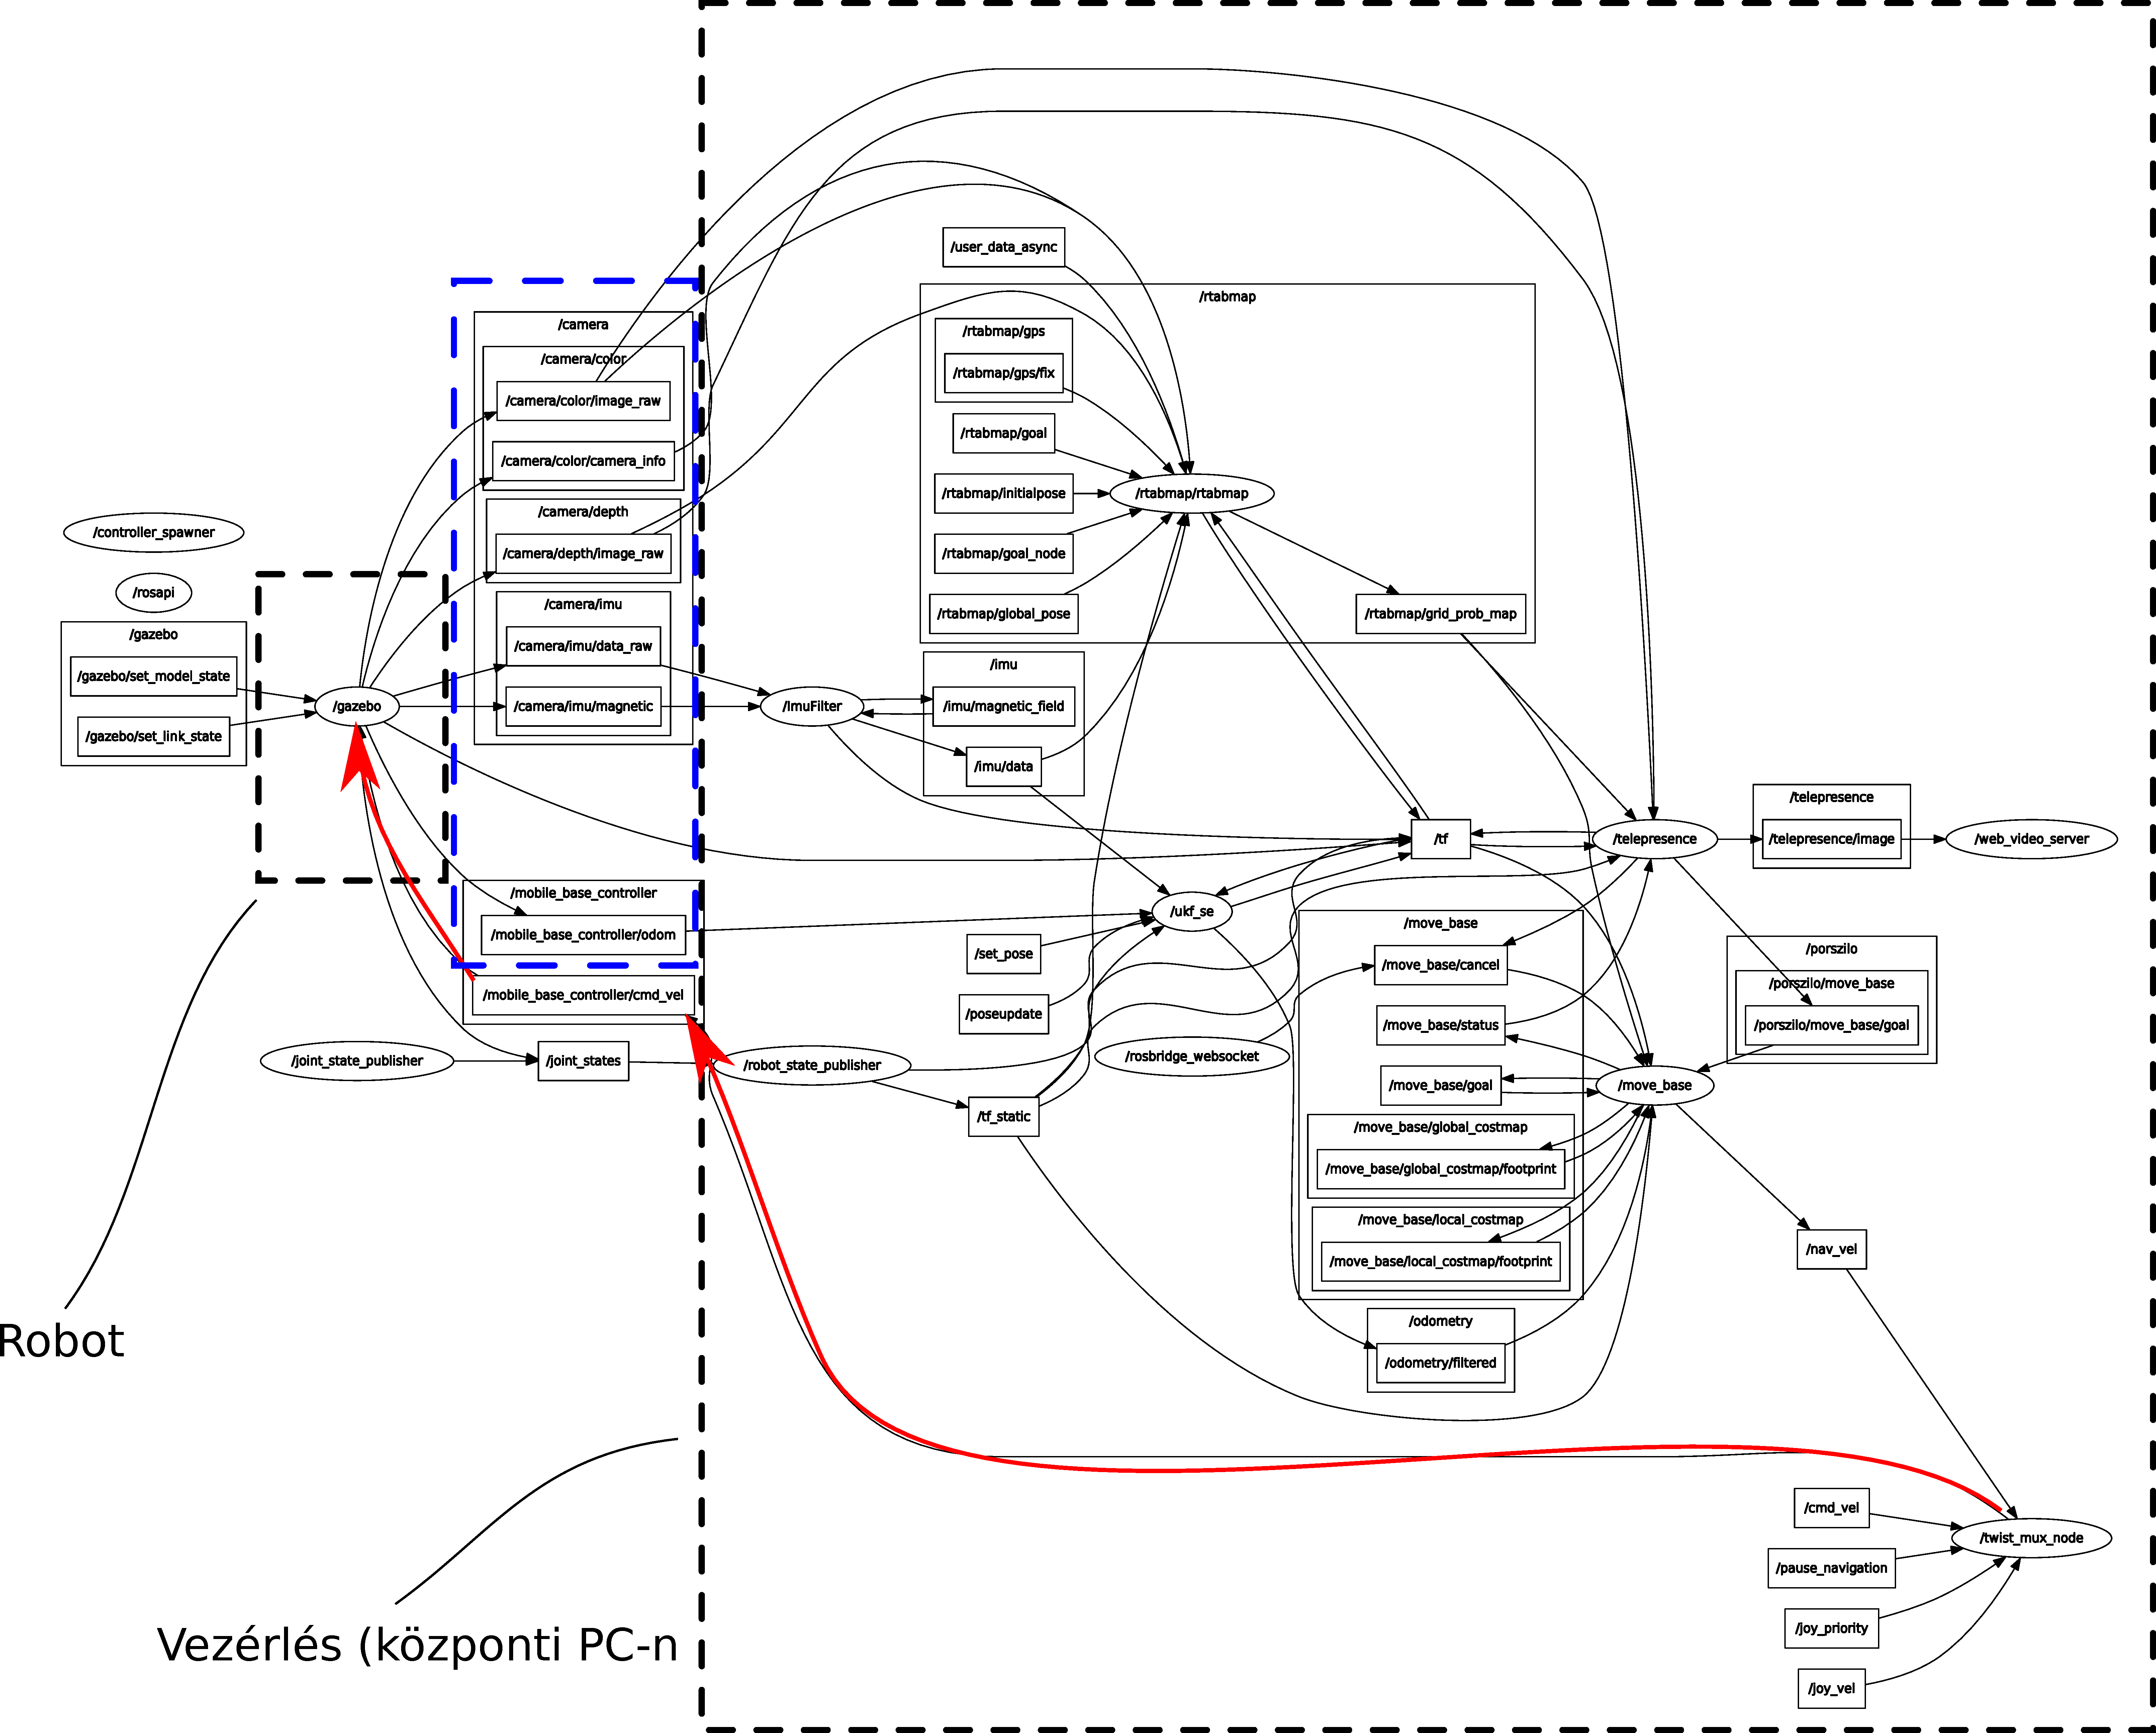
\includegraphics[width=.9\textwidth]{drawn_on}}
\end{figure}
\vspace{\a}
\hrule
\vspace{\a}
A topic-okat bele kell rakni egy \verb|/robotN| namespace-be, hogy valahogy így nézzen ki leegyszerűsítve a dolog:
\begin{figure}[H]
 \centering
 {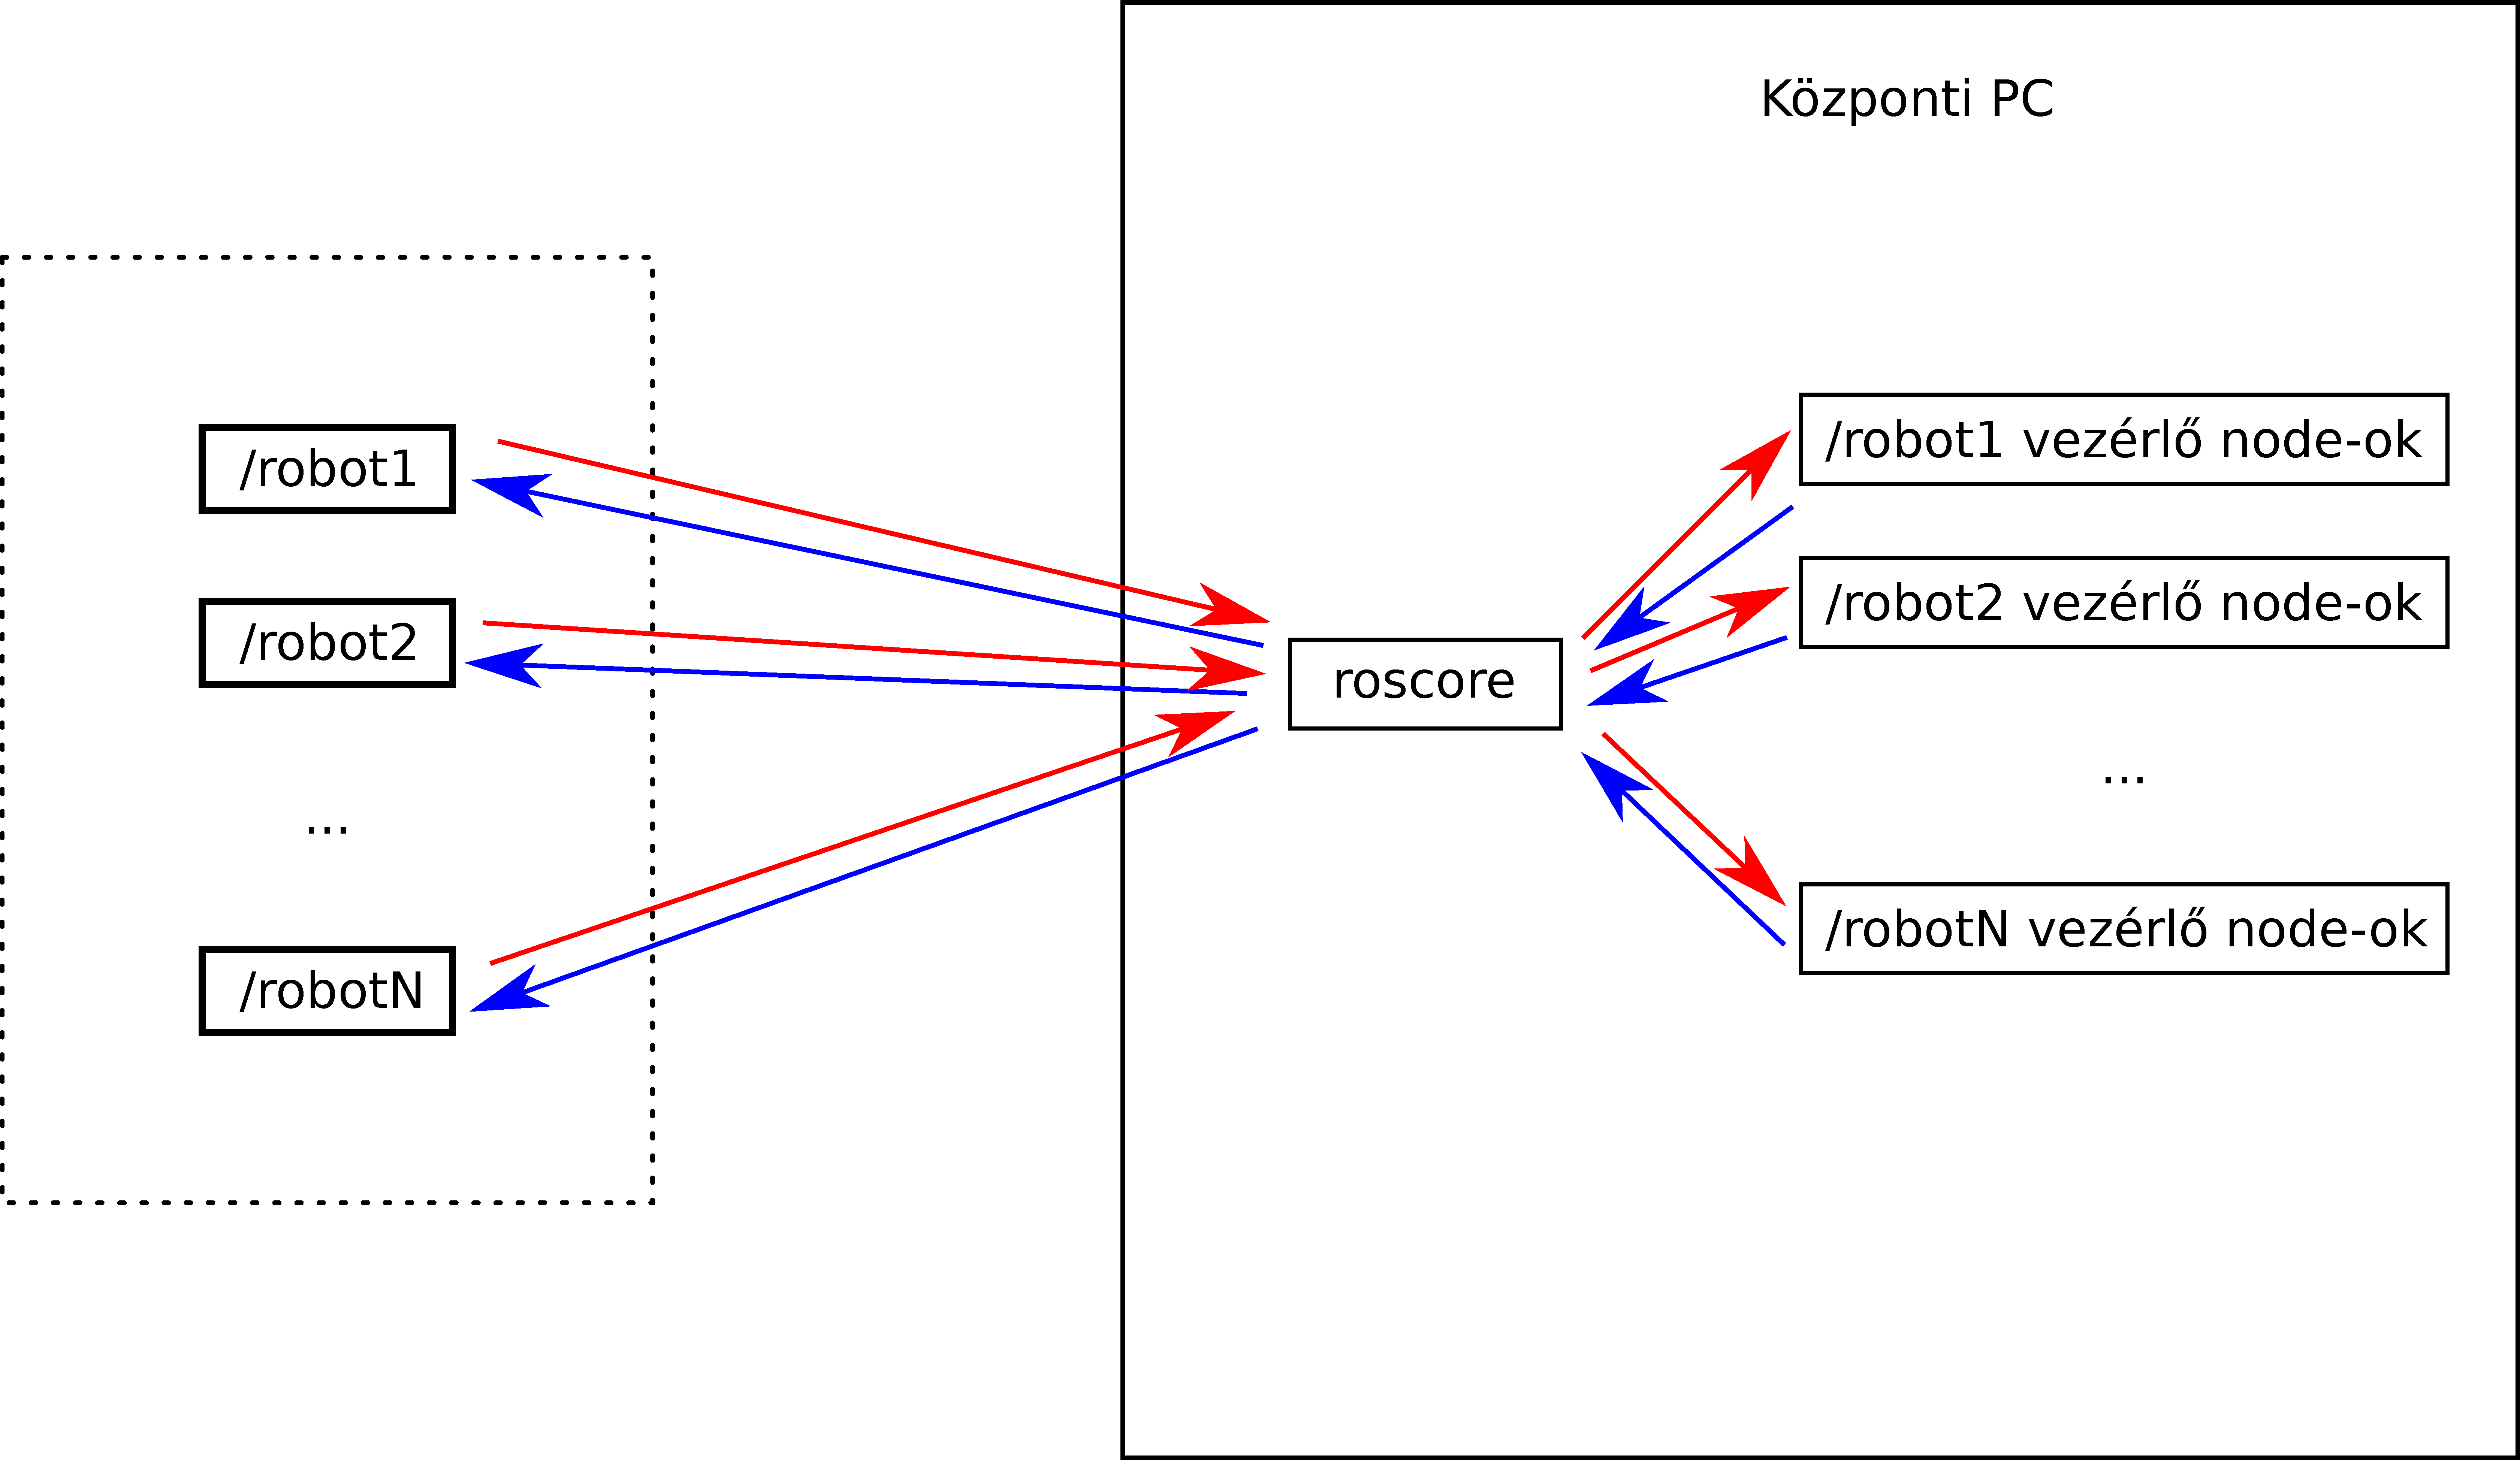
\includegraphics[width=.7\textwidth]{simple}}
\end{figure}
\vspace{\a}
\hrule
\vspace{\a}
Így aztán majd lehet hivatkozni a robotokra, pl. egy belső weboldalon ki tudják majd választani a pincérek hogy melyik robotot szeretnék az adott asztalhoz küldeni, melyik robot hol van, vagy hogy melyik robotot szeretnék telepresence-el irányítani.

\end{document}
